\documentclass[solutions]{esg8012exam} 
  \usepackage{amsmath}
  \usepackage{amssymb}
  \usepackage{enumerate}
  \usepackage{graphicx}
  \usepackage{hyperref}
  \usepackage{siunitx}
  \providecommand{\uvec}[1]{{\hat{\bf{#1}}}}
  \usepackage{pgf,tikz}
  \usetikzlibrary{arrows}
  \usepackage{subfigure}
  %\usepackage{wrapfig}
  \newcommand{\subfigureautorefname}{\figureautorefname}
  \makeatletter
  \newcommand{\interitemtext}[1]{%
    \begin{list}{}
     {\itemindent=0mm\labelsep=0mm
     \labelwidth=0mm\leftmargin=0mm
     \addtolength{\leftmargin}{-\@totalleftmargin}}
      \item #1
    \end{list}
  }
  \makeatother
  \renewcommand{\d}{\,d}
  \providecommand{\norm}[1]{\lVert#1\rVert}
\classname{Physics 8.012} 
\semester{Fall 2010} 
\examnumber{2} 
\date{\today } 
\begin{document}
\section{Problem \thesection\space(30\space points)}
\subsection{Problem}
  A block of mass $m_b$ sits at rest on a frictionless table; the block has a circular surface of radius $R$ as shown in the figure. A small cube of mass $m_c$ and speed $v_{c,0}$ is incident upon the block; the cube slides without friction on the table and slides without friction up the block. At the top of the block, the cube compresses a spring of spring constant $k$ until it momentarily comes to rest a height $R$ above the table. The cube then slides back down until it leaves the block.
  \begin{center}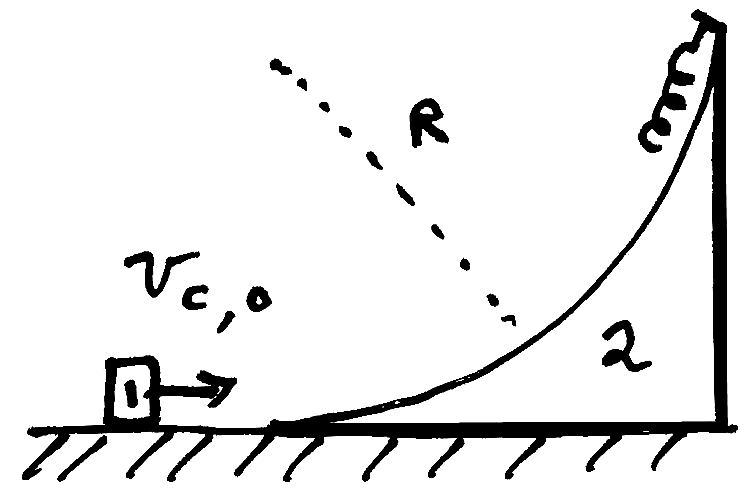
\includegraphics[width=0.35\textwidth]{exam2_p1_1}\end{center}
  \begin{enumerate}[(a)]
    \item How much did the spring compress?
    \item What is the final speed of the block when the cube is no longer on it?
  \end{enumerate}
\subsection{Solution}
  If we take as our system, the cube and block, energy and momentum are both constant since the contact surface is frictionless and normal forces do no work. When the cube has reached its maximum height, the cube and block are moving with the same final speed $v_1$.
  \begin{center}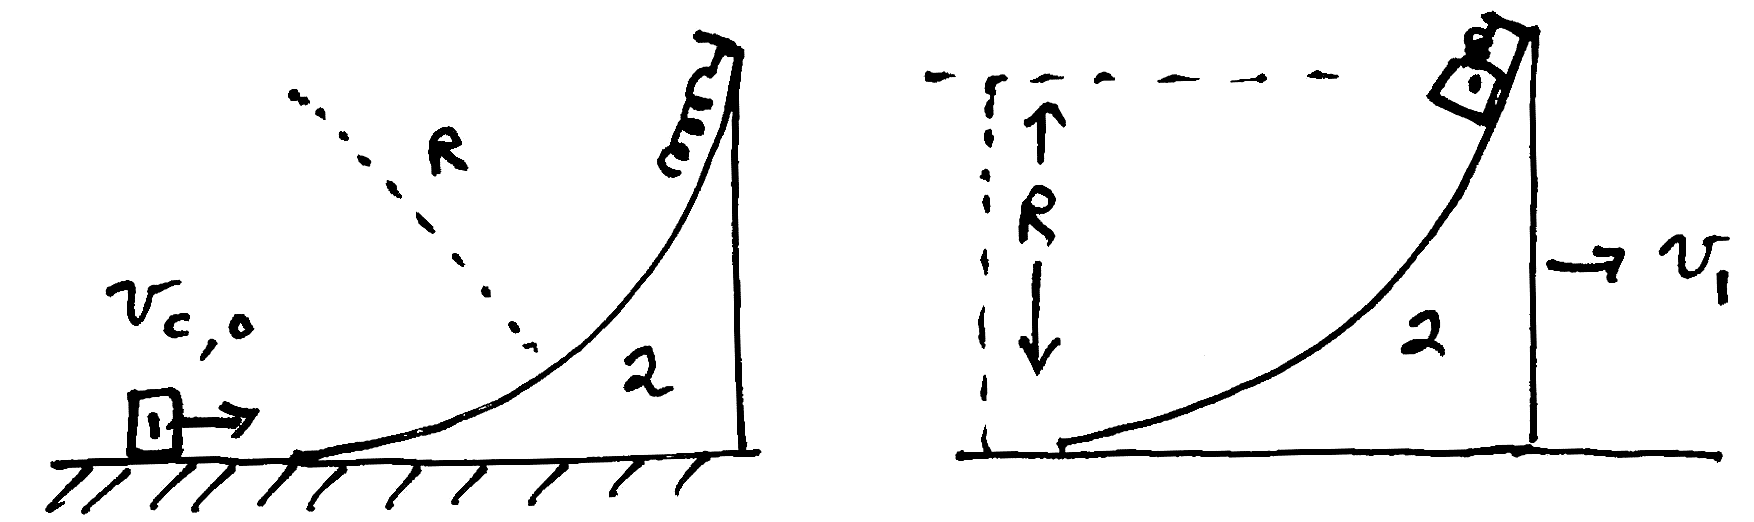
\includegraphics[width=0.9\textwidth]{exam2_s1_1}\end{center}
  Therefore the momentum of the system is
  \begin{equation} m_c v_{c,0} = (m_c + m_b) v_1 \label{eq:1:system_momentum} \end{equation}
  which we can solve for the speed of the cube and block when the cube is at rest relative to the block.
  \begin{equation} v_1 =  \frac{m_c v_{c, 0}}{m_c + m_b}. \label{eq:1:v_1} \end{equation}
  The energy of the system is
  \begin{equation} \frac12 m_c v_{c,0}^2 = \frac12 (m_c + m_b)v_1^2 + m_c g R + \frac12 k x_f^2 \label{eq:1:system_energy} \end{equation}
  Substituting \autoref{eq:1:v_1} into the energy condition yields
  \begin{equation} \frac12 m_c v_{c,0}^2 = \frac12 (m_c + m_b)\left( \frac{m_c v_{c,0}}{m_c + m_b}\right)^2 + m_c g h + \frac12 k x_f^2. \label{eq:1:system_energy_2} \end{equation}
  We can rewrite this in terms of the change in potential energy
  \begin{align}
    \Delta U & = \frac12 k x_f^2 + m_c g R = \frac12 m_c v_{c,0}^2 - \frac12 (m_c + m_b) \left( \frac{m_c v_{c,0}}{m_c + m_b}\right)^2 = \frac12 m_c v_{c, 0}^2\left( 1 - \frac{m_c}{m_c + m_b}\right) \nonumber \\
    & = \frac12 \frac{m_c m_b}{m_c + m_b} v_{c,0}^2 = \frac12 \mu v_{c,0}^2 \label{eq:1:potential_energy}
  \end{align}
  where
  \begin{equation} \mu \equiv \frac{m_c m_b}{m_c + m_b} \label{eq:1:def_mu} \end{equation}
  is the reduced mass. This should not be surprising. Because the collision is elastic,
  \begin{equation} \Delta U = -\Delta K = -\left(\frac12 \mu v_{\text{rel},f}^2 - \frac12 \mu v_{\text{rel},0}^2\right). \label{eq:1:delta_U=-delta_K} \end{equation}
  The final relative speed is $v_{\text{rel}, f} = 0$ and the initial relative speed is $v_{\text{rel}, 0} = v_{c, 0}$, so \autoref{eq:1:delta_U=-delta_K} becomes
  \begin{equation} \frac12 k x_f^2 + m_c g R = \frac12\mu v_{c,0}^2 \label{eq:1:energy_substituted} \end{equation}
  in agreement with \autoref{eq:1:potential_energy}. So the amount that the spring was compressed is
  \begin{equation} x_f = \sqrt{\frac{\mu v_{c,0}^2 - 2m_c g h}{k}}. \label{eq:1:x_f} \end{equation}
  We show the momentum diagram when the cube comes back down the block along with the momentum diagram before the cube went up the block in the figure below.
  \begin{center}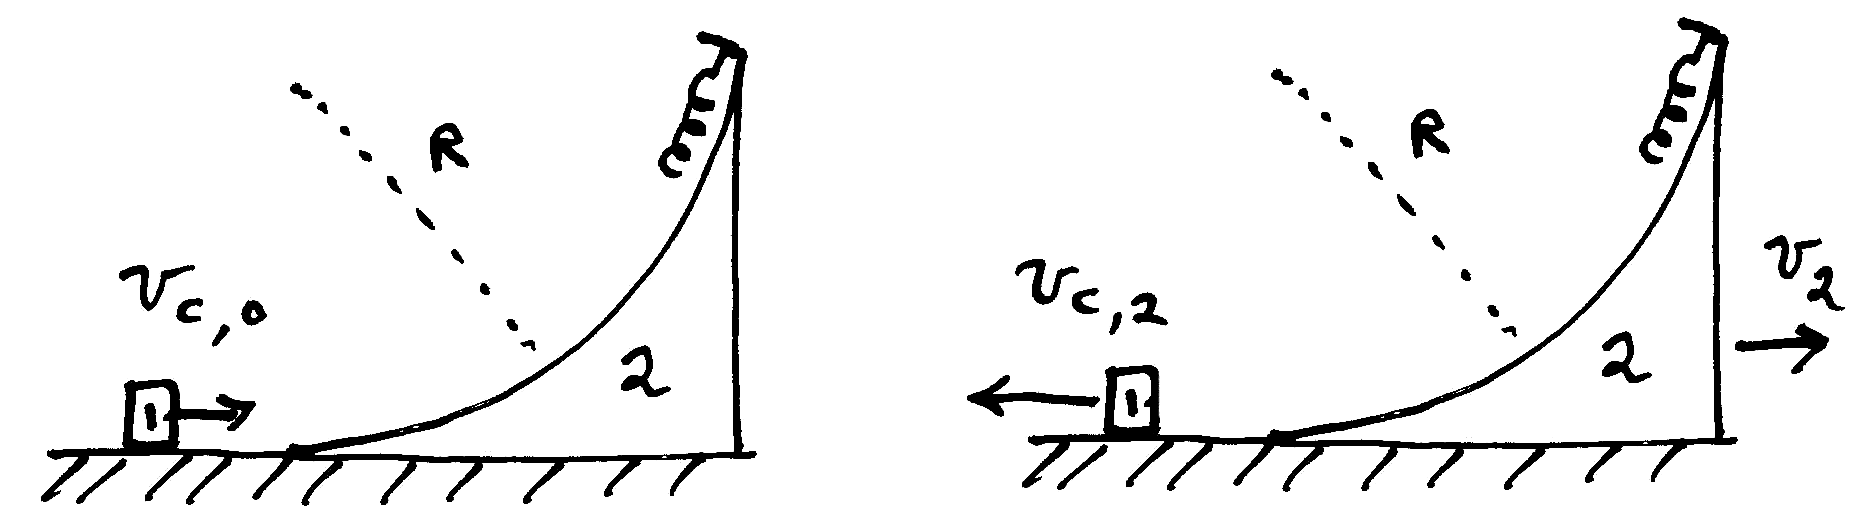
\includegraphics[width=0.9\textwidth]{exam2_s1_2}\end{center}
  We can again apply the condition that the momentum of the system is constant,
  \begin{equation} m_c v_{c,0} = m_b v_{b, 2} - m_c v_{c, 2} \label{eq:1:constant_momentum} \end{equation}
  which can be rewritten as
  \begin{equation} m_c(v_{c,0} + v_{c, 2}) = m_b v_{b,2}. \label{eq:1:momentum_constant_rewritten} \end{equation}
  The condition that the energy of the system is constant becomes
  \begin{equation} \frac{1}{2}m_c v_{c,0}^2=\frac{1}{2}m_c v_{c,2}^2+\frac{1}{2}m_b v_{b,2}^2. \label{eq:1:constant_energy} \end{equation}
  We can rewrite the energy equation as
  \begin{equation} m_c (v_{c,0}^2-v_{c,2}^2)=m_b v_{b,2}^2 \label{eq:1:constant_energy_rewritten} \end{equation}
  which after factoring becomes
  \begin{equation}
  m_c (v_{c,0} -v_{c,2} )(v_{c,0} +v_{c,2} )=m_b v_{b,2}^2. \label{eq:1:constant_energy_factored} \end{equation}
  Dividing \autoref{eq:1:constant_energy_factored} by \autoref{eq:1:momentum_constant_rewritten} yields
  \begin{equation} (v_{c,0} -v_{c,2} )=v_{b,2} \label{eq:1:energy_momentum_combined_1} \end{equation}
  or
  \begin{equation} v_{c,2} =v_{c,0} -v_{b,2}. \label{eq:1:energy_momentum_combined_2} \end{equation}
  Note that \autoref{eq:1:energy_momentum_combined_2} can be rewritten as $v_{c,0} =v_{b,2} +v_{c,2}$ which is just our condition that the relative speed remains unchanged $v_{rel,0} =v_{rel,2}$. We can substitute \autoref{eq:1:energy_momentum_combined_2} into \autoref{eq:1:constant_momentum} and find that
  \begin{equation} m_c v_{c,0} = m_b v_{b,2} - m_c(v_{c,0} - v_{b,2}). \label{eq:1:momentum_c_0} \end{equation}
  We can solve \autoref{eq:1:momentum_c_0} for the speed of the block when the cube leaves the block,
  \begin{equation} v_{b, 2} = \frac{2m_c v_{c,0}}{m_b + m_c}. \label{eq:1:v_b2} \end{equation}
  Suppose we view the condition from the center of mass frame.
  \begin{center}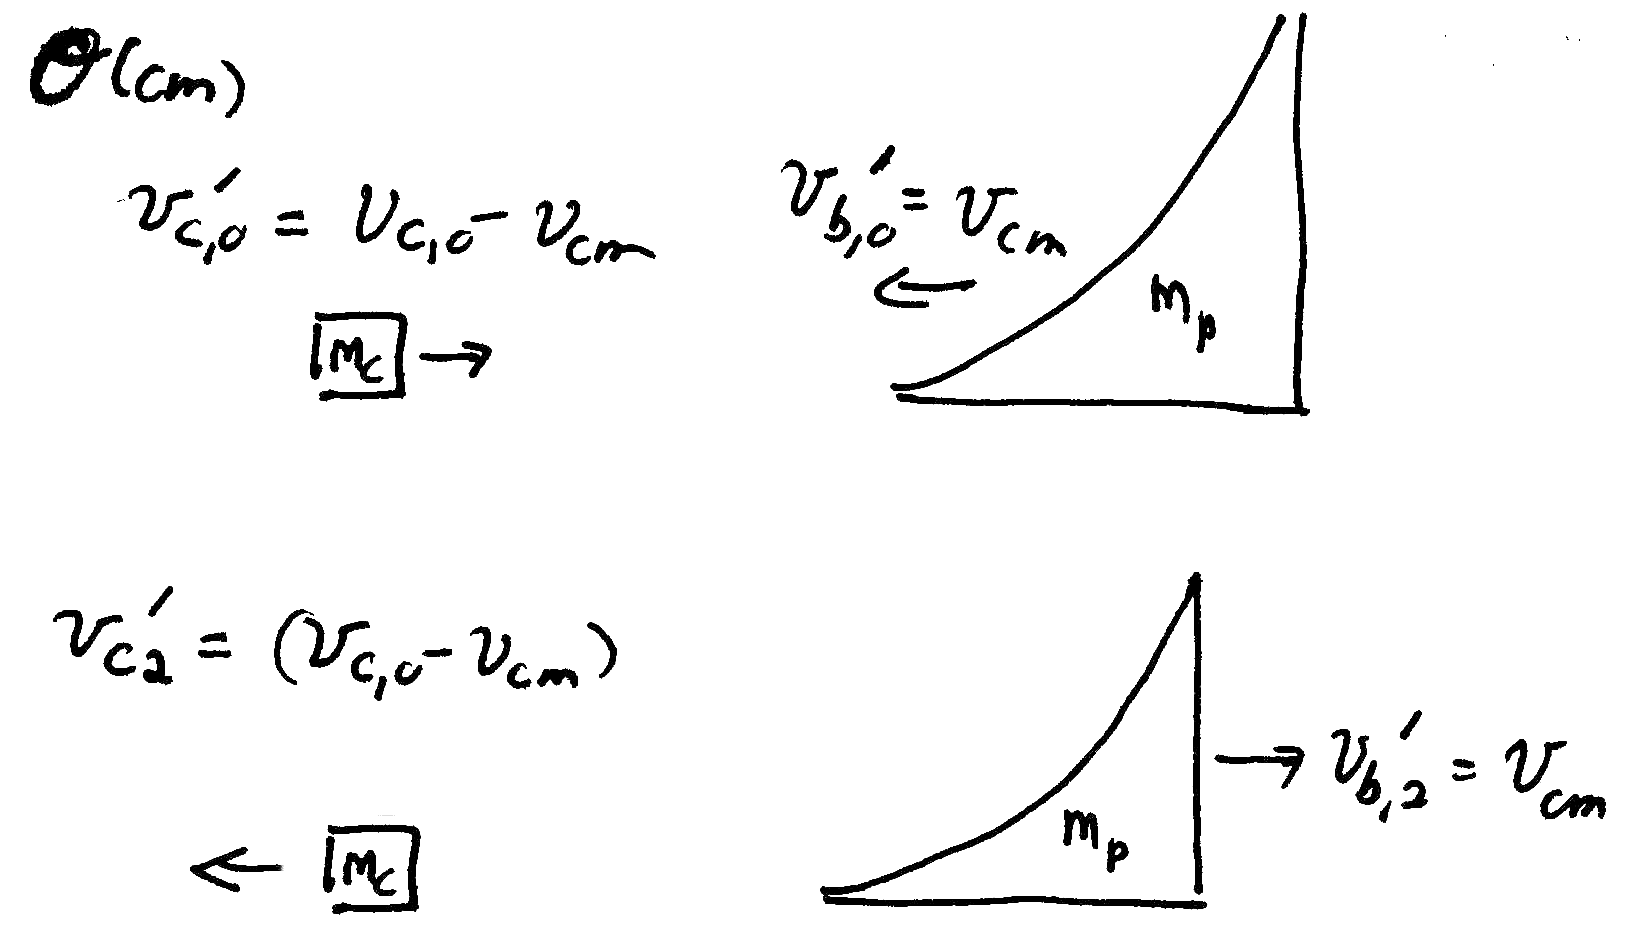
\includegraphics[width=0.6\textwidth]{exam2_s1_3}\end{center}
  Then the block has an initial speed equal to the center of mass speed
  \begin{equation} {v}'_{b,0} =\frac{m_c v_{c,0} }{m_b +m_c }. \label{eq:1:v_b0'} \end{equation}
  After the collision the block reverses direction but maintains the same speed in the center of mass frame so
  \begin{equation} {v}'_{b,2} ={v}'_{b,0} =\frac{m_c v_{c,0} }{m_b +m_c }. \label{eq:1:v_b2'} \end{equation}
  In the lab frame the speed of the block is then
  \begin{equation} v_{b,2} ={v}'_{b,2} +v_{cm} =\frac{m_c v_{c,0} }{m_b +m_c }+\frac{m_c v_{c,0} }{m_b +m_c }=\frac{2m_c v_{c,0} }{m_b +m_c }.\label{eq:1:v_b2} \end{equation}
  This is in agreement with \autoref{eq:1:v_b2}.
\clearpage
\section{Problem \thesection\space(35\space points)}
\subsection{Problem}
  A particle initially sits on top of a large smooth sphere of radius $R$ as shown in the figure. The particle begins to slide along the surface of the sphere. There is a friction force between the particle and the surface that varies with the angle $\theta$ according to
  $$f = f_0\sin\theta$$
  where $f_0$ is a constant. Let $g$ denote the gravitational constant.
  \begin{center}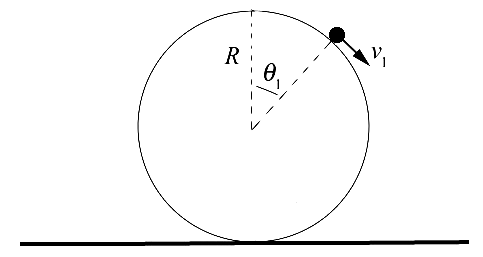
\includegraphics[width=0.3\textwidth]{exam2_p2_1}\end{center}
  \begin{enumerate}[(a)]
    \item Determine the angle $\theta_1$ with respect to the vertical at which the particle will lose contact with the surface of the sphere.
    \item What is the speed $v_1$ of the particle at the instant it loses contact with the surface of the sphere.
  \end{enumerate}
\subsection{Solution}
  \begin{enumerate}[(a)]
    \item Since the particle slides down the sphere, and friction always points opposite the direction of motion, the free body diagram for the particle when it is at an angle $\theta$ is
      \begin{center}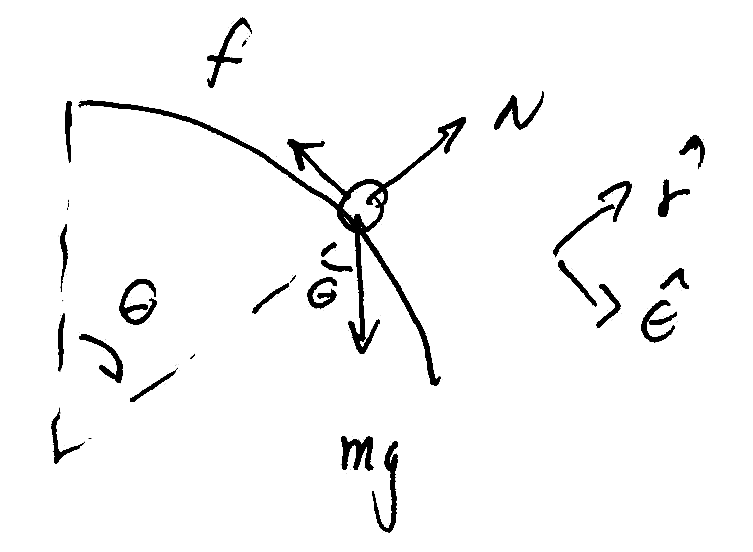
\includegraphics[width=0.35\textwidth]{exam2_s2_1}\end{center}
      So long as the particle remains on the surface of the sphere, it moves in a circle, and $F = ma$ in the $\hat r$ direction is
      \begin{equation*} N - m g \cos\theta = -\frac{mv^2}{R}. \end{equation*}
      The instant the particle looses contact with the sphere is the instant $N = 0$.  Plugging this in to our equation above,
      \begin{equation*} -mg \cos\theta_1 = -\frac{mv_1^2}{R}. \end{equation*}% \label{eq:2:F=ma_loose_contact}
      Multiplying both sides by $-R / 2$,
      \begin{equation} \frac12 m v_1^2 = \frac{R mg \cos\theta_1}{2}. \label{eq:2:F=ma_loose_contact_changed} \end{equation}
      Now apply conservation of energy.  Defining $U$ to be zero when $\theta = \theta_1$, we get
      \begin{center}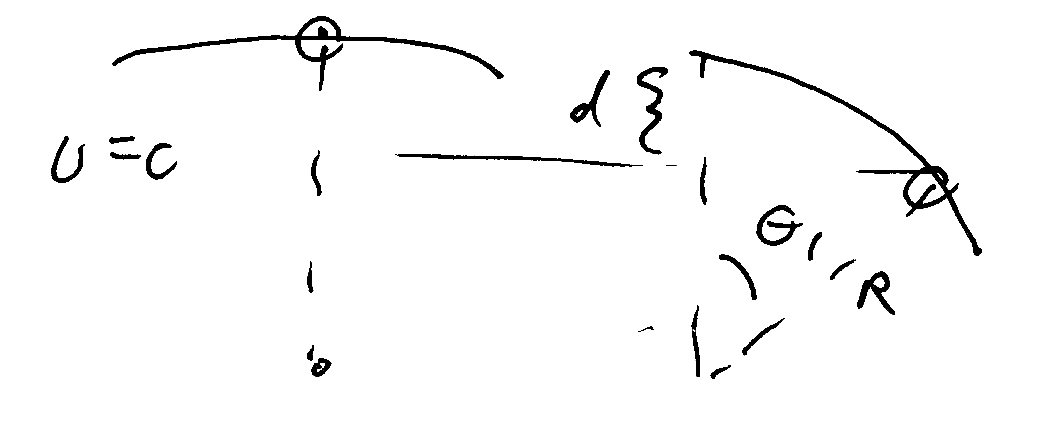
\includegraphics[width=0.35\textwidth]{exam2_s2_2}\end{center}
      where $d = R(1 - \cos\theta_1)$.

      Calculating the initial and final kinetic and potential energies,
      \begin{align*}
        K_i & = 0                           & K_f & = \frac12 m v_1^2 \\
        U_i & = mgd = mgR(1 - \cos\theta_1) & U_f & = 0
      \end{align*}
      Since work is defined to be $\int \vec F \cdot d\vec s$, we can calculate the word done by friction to be
      \begin{align*}
        W & = \int -f_0\sin\theta\,ds \\
          & = -\int_{0}^{\theta_1} f_0\sin\theta R,\d\theta \\
          & = \left. f_0\cos\theta R\right|_0^{\theta_1} \\
          & = f_0 R(\cos\theta_1 - 1)
      \end{align*}
      Since friction is the only non-conservative force, we also have that the work done by friction is the change in energy,
      \begin{equation*} W = E_f - E_i = \frac12 m v_1^2 - mgR(1 - \cos\theta_1). \end{equation*}
     Combining these equations,
    \begin{equation*} f_0 R(\cos\theta_1 - 1) = \frac12 m v_1^2 - m g R(1 - \cos\theta_1).\end{equation*}
    Plugging in our expression for $\frac12 m v_1^2$ from \autoref{eq:2:F=ma_loose_contact_changed}, this becomes
    \begin{equation*} f_0 R(\cos\theta_1 - 1) = \frac{R mg \cos\theta_1}{2} - m g R(1 - \cos\theta_1).\end{equation*}
    Bringing all the terms with $\cos\theta_1$ to the left hand side and factoring,
    \begin{equation*} R\cos\theta_1\left(f_0 - \frac32 m g\right) = R(f_0 - m g). \end{equation*}
    Solving for $\cos\theta_1$ gives us
    \begin{equation*} \cos\theta_1 = \frac{f_0 - m g}{f_0 - \frac32 m g}. \end{equation*}
  \item Division of both sides of \autoref{eq:2:F=ma_loose_contact_changed} yields
    \begin{equation*} v_1^2 = g R \cos\theta_1. \end{equation*}
    Plugging in $\cos\theta_1$ and taking the square root of both sides,
    \begin{equation*} v_1 = \sqrt{g R \left(\frac{f_0 - m g}{f_0 - \frac32 m g}\right)}. \end{equation*}
  \end{enumerate}
\clearpage
\section{Problem \thesection\space(35\space points)}
\subsection{Problem}
  \begin{center}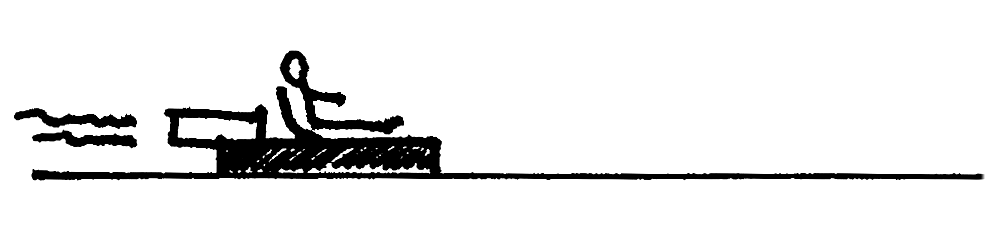
\includegraphics[width=0.6\textwidth]{exam2_p3_1}\end{center}
  A rocket sled ejects gas backwards at a speed $u$ relative to the rocket sled. The mass of the fuel in the rocket sled is equal to one half the initial total mass $m_{r,0}$ (including fuel) of the sled.  The rocket sled starts from rest on a frictionless track. You may ignore air resistance.
  \begin{enumerate}[(a)]
    \item Derive a relation between the differential of the speed of the rocket sled, $dv$, and the differential of the total mass of the rocket, $dm_r$.
    \item Integrate the above relation to find the speed of the rocket sled as a function of mass, $v_r(m)$, as the rocket sled speeds up.
    \item What is the final speed of the rocket sled after all the fuel has been burned?  Express your answers in terms of the quantities $u$, and $m_{r,0}$ as needed.
    \item After reaching its final speed, the sled enters a rough portion of the track that begins at $x=0$ with a coefficient of kinetic friction that varies with distance $\mu_k(x) = bx$ where $b$ is a positive constant.  How far $D$ did the sled slide before it came to rest in that portion of the track? Express your answers in terms of the quantities $u$, $b$, and $m_0$ as needed.
  \end{enumerate}
\subsection{Solution}
  \begin{enumerate}[(a)]
    \item
      Take as the system the rocket sled, fuel, and the small amount of fuel of mass $\Delta m_f$ that is ejected during the interval $[t, t + \Delta t]$. Let the positive $x$-direction be to the right in the figures below. We first show the momentum diagram at time $t$:
      \begin{center}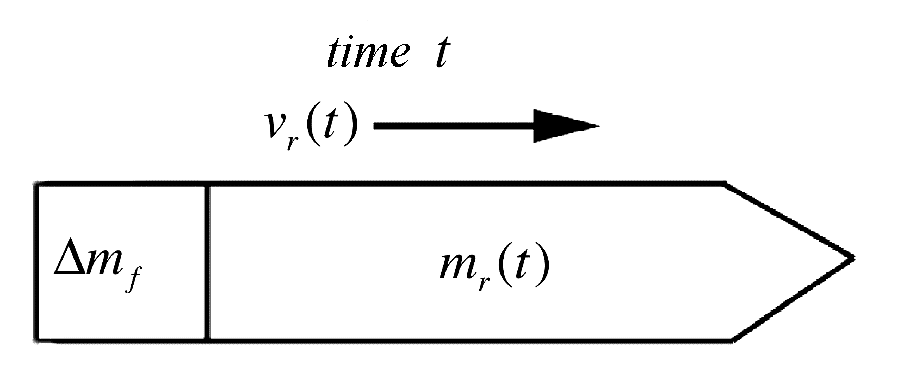
\includegraphics[width=0.6\textwidth]{exam2_s3_1}\end{center}
      The smaller square represents the small amount of fuel of mass $\Delta m_f$ that is ejected during the interval $[t,t+\Delta t]$. In the above figure $m_r (t)$ is the combined mass of the rocket sled, the dry mass of the rocket sled plus the mass of fuel inside the rocket sled at time $t$ that does not leave the rocket sled during the interval. The $x$-component of the velocity of the rocket sled is denoted by $v_r(t)$.  In analyzing our momentum diagrams we shall drop the explicit reference to time dependence for the mass of the rocket and the $x$-component of the velocity of the rocket sled, denoting them respectively by $m_r$ and $v_r $. Returning to our momentum diagram we see that at time $t$, the $x$-component of the momentum of the system $p_x^\text{sys}(t)$ is given by
      \begin{equation} p_x^\text{sys}(t)=(m_r +\Delta m_f) v_r  \label{eq:3:p_x^sys(t)} \end{equation}
      By the end of the interval the rocket has recoiled forward with $x$-component of the velocity $v_r +\Delta v_r $. The fuel is ejected backwards relative to the rocket sled with speed $u$, hence with a speed $v_r +\Delta v_r -u$ relative to the fixed reference frame depicted in the figures. After the interval has ended the momentum diagram of the system is shown below.
      \begin{center}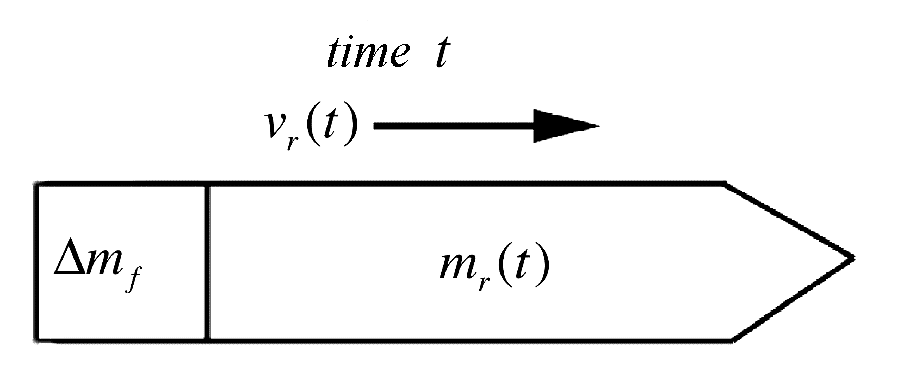
\includegraphics[width=0.6\textwidth]{exam2_s3_1}\end{center}
      At time $t+\Delta t$, the $x$-component of the momentum of the system $p_x^\text{sys} (t+\Delta t)$ is given by
      \begin{equation} p_x^\text{sys} (t+\Delta t) = m_r (v_r +\Delta v_r )+\Delta m_f (v_r +\Delta v_r -u) \label{eq:3:p_x^sys(t+delta_t)} \end{equation}
      and so the change in $x$-component of the momentum of the system during the interval $[t,t+\Delta t]$ is
      \begin{align}
        \Delta p_x^\text{sys} & = p_x^\text{sys} (t+\Delta t)-p_x^\text{sys} (t) \nonumber \\
          & = m_r (v_r +\Delta v_r )+\Delta m_f (v_r +\Delta v_r -u)-(m_r +\Delta m_f )v_r \nonumber \\
          & = m_r \Delta v_r +\Delta m_f \Delta v_r -\Delta m_f u. \label{eq:3:delta_p_x^sys}
      \end{align}
      There are no external forces acting in the $x$-direction, therefore the momentum principle
      \begin{equation} F_x^\text{ext} =\lim_{\Delta t\to 0} \frac{\Delta p_x^\text{sys} }{\Delta t} \label{eq:3:F_x^ext=lim} \end{equation}
      becomes
      \begin{equation} 0 = \lim_{\Delta t\to 0} \frac{m_r \Delta v_r +\Delta m_f \Delta v_r -\Delta m_f u}{\Delta t}. \label{eq:3:expanded_F_ext} \end{equation}
      We note that
      \begin{equation} \lim_{\Delta t\to 0} \frac{\Delta m_f \Delta v_r }{\Delta t}=0. \label{eq:3:second_order_differential_zero} \end{equation}
      Then using the definition of the derivative, we find that the differential equation describing the motion of the system is given by
      \begin{equation} 0=m_r \frac{dv_r }{dt}-\frac{dm_f }{dt}u \label{eq:3:diff_eq_m_v} \end{equation}
      Because the fuel is being ejected at a positive rate and the mass of the rocket sled is the rate of decrease of the mass of the rocket sled is  negative we have that
      \begin{equation} \frac{dm_r }{dt}=-\frac{dm_f }{dt} \label{eq:3:dmr_dmf} \end{equation}
      We can now substitute \autoref{eq:3:dmr_dmf} into \autoref{eq:3:diff_eq_m_v} and find that
      \begin{equation} 0=m_r \frac{dv_r }{dt}+\frac{dm_r }{dt}u. \label{eq:3:diff_eq_mr_v} \end{equation}
      We can solve this equation by the technique of separation of variables.  First rewrite the equation as
      \begin{equation} m_r \frac{dv_r }{dt}=-\frac{dm_r }{dt}u. \label{eq:3:separation_of_variables_v_mr_1} \end{equation}
      Multiple each side by $dt$ and divide by through by $m_r $. Thus
      \begin{equation} dv_r =-\frac{dm_r }{m_r }u. \label{eq:3:separation_of_variables_v_mr_2} \end{equation}
    \item \emph{Integrate the above relation to find the speed of the rocket sled as a function of mass, $v(m)$, as the rocket sled speeds up.} \par
      We can integrate both sides of \autoref{eq:3:separation_of_variables_v_mr_2}
      \begin{equation} \int_{v_r =0}^{v_{r,f} } {dv_r } =-u\int_{m_{r,0} }^{m_{r,0} } {\frac{dm_r }{m_r }} . \label{eq:3:integration_vr_mr} \end{equation}
      Integration yields
      \begin{equation} v_{r,f} =-u\ln \left( {\frac{m_{r,f} }{m_{r,0} }} \right)=u\ln \left( {\frac{m_{r,o} }{m_{r,f} }} \right) \label{eq:3:vrf}\end{equation}
    \item \emph{What is the final speed of the rocket sled after all the fuel has been burned? Express your answers in terms of the quantities $u$, and $m_{r,0}$ as needed.} \par
      Because $m_{r,f} =\frac12m_{r,0}$, the final speed of the rocket sled after the fuel has been burned is
      \begin{equation} v_{r,f} =u\ln 2 \label{eq:3:vf_u} \end{equation}
    \item \emph{After reaching its final speed, the sled enters a rough portion of the track that begins at $x=0$ with a coefficient of kinetic friction that varies with distance $\mu_k (x)=bx$ where $b$ is a positive constant. How far $D$ did the sled slide before it came to rest in that portion of the track? Express your answers in terms of the quantities $u$, $b$, and $m_0$ as needed.} \par
      \begin{center}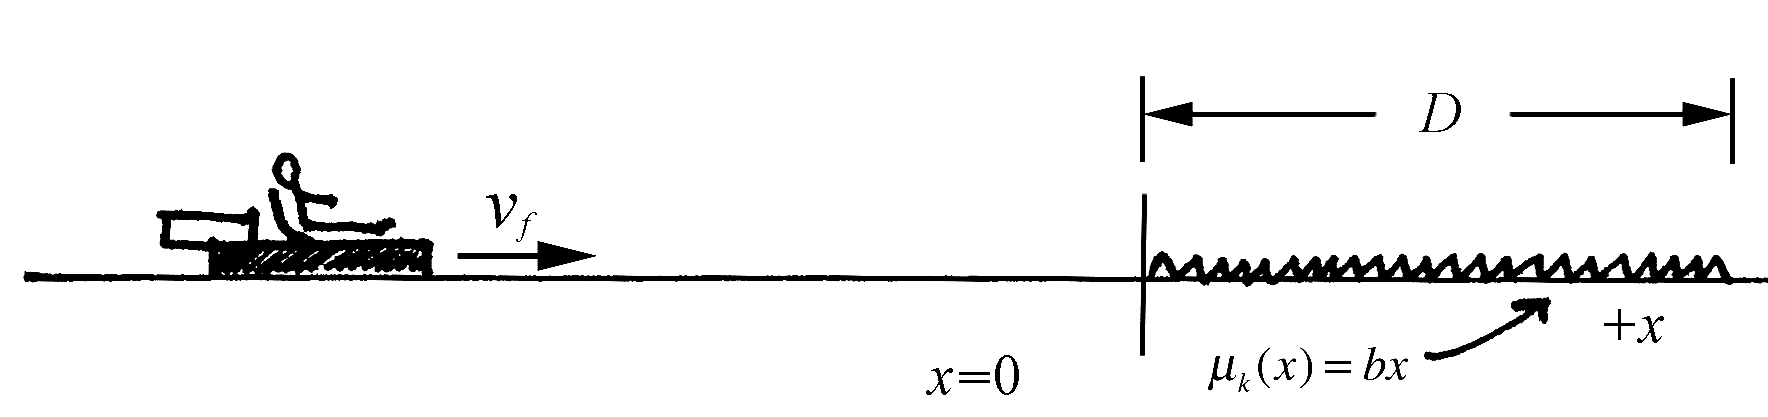
\includegraphics[width=0.9\textwidth]{exam2_s3_3}\end{center}
      We shall use the energy law that
      \begin{equation} W_\text{nc} =E_f -E_i . \label{eq:3:Wnc} \end{equation}
      The non-conservative work is due to friction
      \begin{equation} W_\text{nc} =-\int_0^D {f_k } dx=-m_{r,0} g\int_0^D {\mu_k (x)} dx=-m_{r,0} g\int_0^D {bx} dx=-m_{r,0} gb(D^2/2) \label{eq:3:Wnc_friction} \end{equation}
      The final mechanical energy is zero,
      \begin{equation} E_f =0 \label{eq:3:Ef=0} \end{equation}
      and the initial mechanical energy is just the kinetic energy of the sled after the fuel as been burned,
      \begin{equation} E_i =\frac{1}{2}m_{r,f} v_{r,f}^2=\frac{m_{r,0} u\ln 2}{4}. \label{eq:3:E_i} \end{equation}
      Substituting \autoref{eq:3:Wnc_friction}, \autoref{eq:3:Ef=0}, and \autoref{eq:3:E_i} into \autoref{eq:3:Wnc} yields
      \begin{equation} -m_{r,0} gb(D^2/2)=-\frac{m_{r,0} u\ln 2}{4}. \label{eq:3:energy_constraint_substituted} \end{equation}
      We can solve \autoref{eq:3:energy_constraint_substituted} for the distance $D$ that the sled slid before it came to rest
      \begin{equation} D=\sqrt {\frac{u\ln 2}{2gb}} . \label{eq:3:D} \end{equation}
  \end{enumerate}
\clearpage
\end{document}
